% ---------------------------------------------------------------------
% Cloned from the HES-SO//Master canvas 2019
% ---------------------------------------------------------------------


\chapter{Experiments \& Results}
\label{chap:experiments-results}
\section{Environments}
\subsection{Jupyter Notebook}
\subsection{Local Machine}
\subsection{Amazon Web Services}
\subsection{iColab-gpu2}
\subsection{CPU Dedicated Machine}


\section{Gensim Framework}
\paragraph{Errors} Memory allocation with multi-core. The problem is occurring during the merge of the cores. Indeed, my current machine has 128GB ram, and the dataset weights about 16GB in the memory, and each core during merging is processing at least the same amount, plus the processed informations.\\ 

\begin{figure}[htbp]
\centering
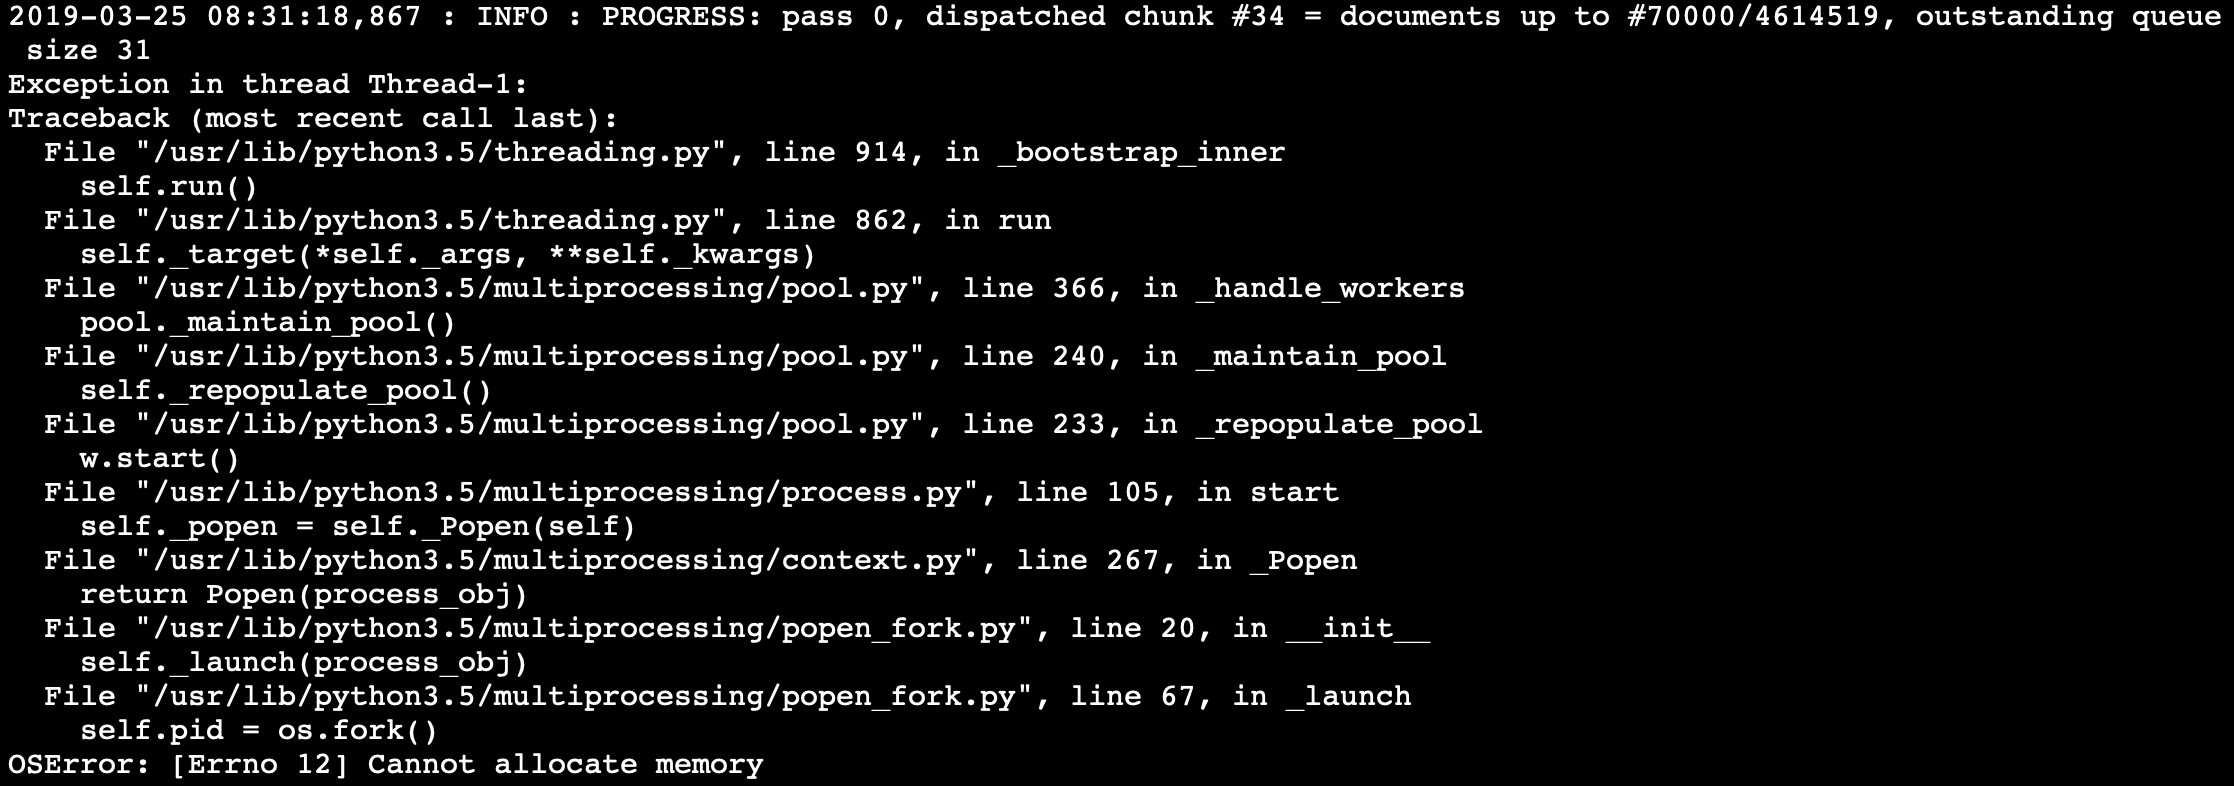
\includegraphics[width=\linewidth]{99-imgs/gensim_memory_allocation_error}
\caption{Error 1}
\label{fig:error-1}
\end{figure}

\begin{figure}[htbp]
\centering
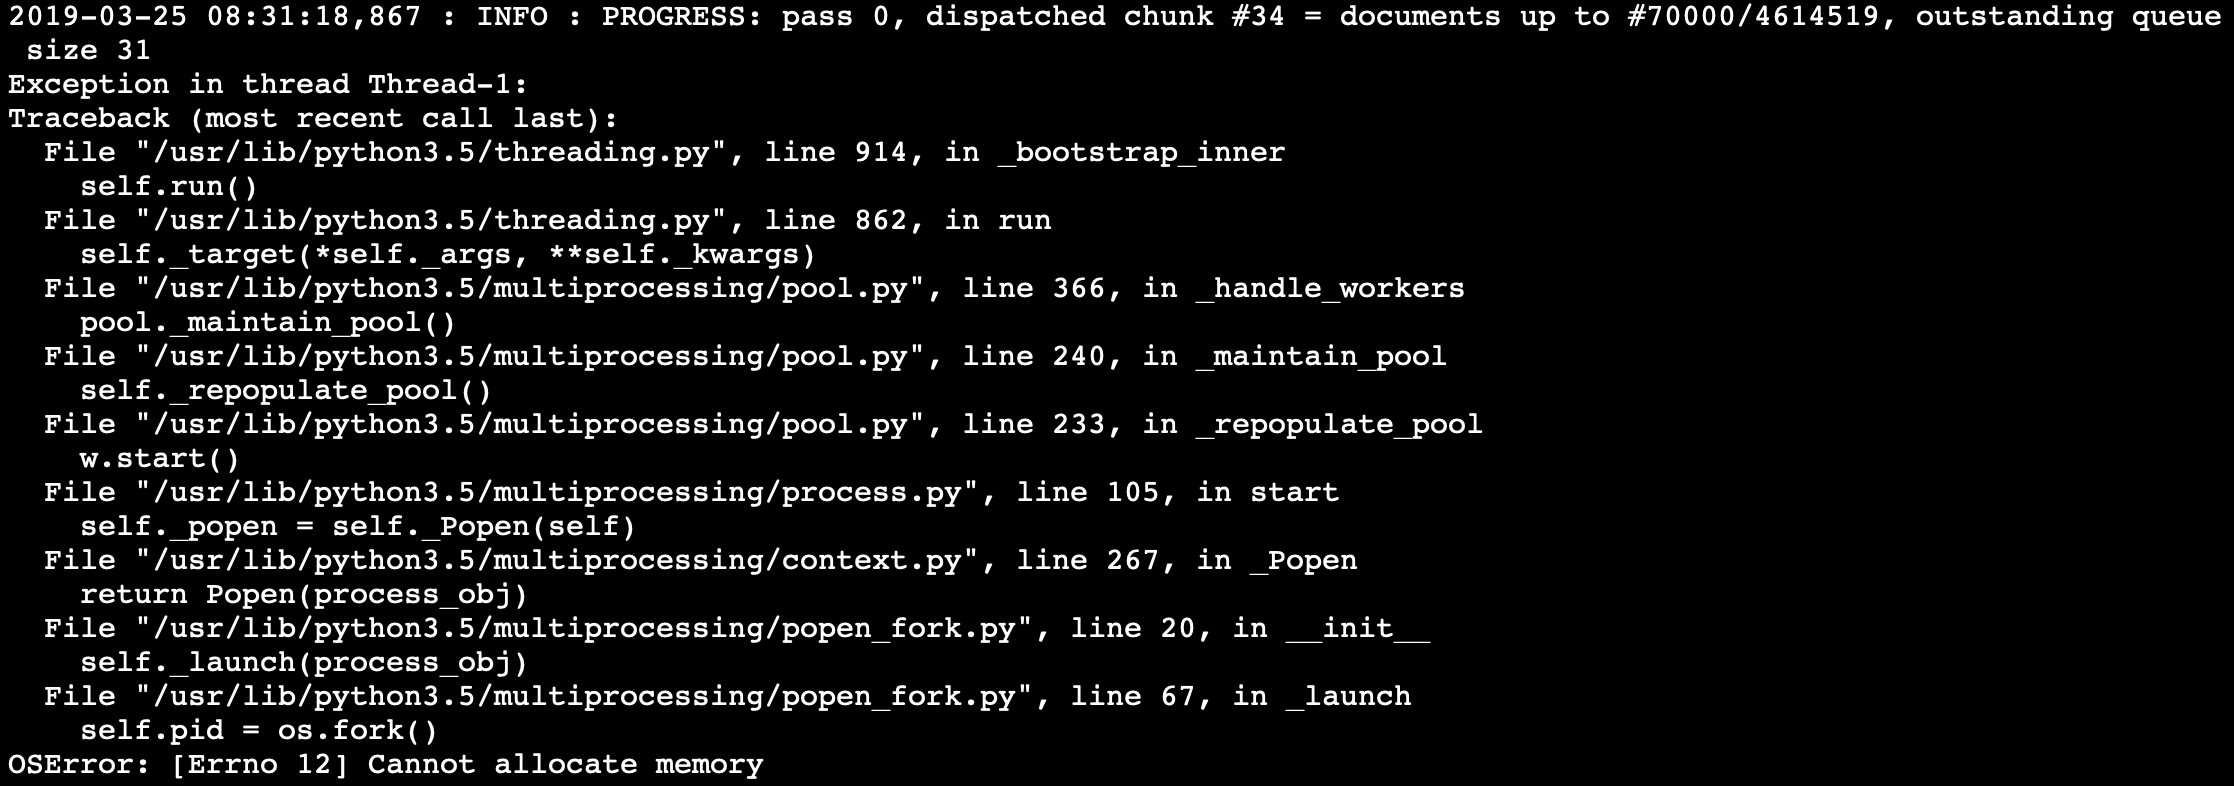
\includegraphics[width=\linewidth]{99-imgs/gensim_memory_allocation_error}
\caption{Error 2}
\label{fig:error-2}
\end{figure}

\section{Materials}

\section{Products}



